\section{Results} \label{sec:results}

\subsection{Download Performance: Latency vs. Throughput}

\begin{figure}[H]
    \centering
    \begin{subfigure}{0.48\textwidth}
        \centering
        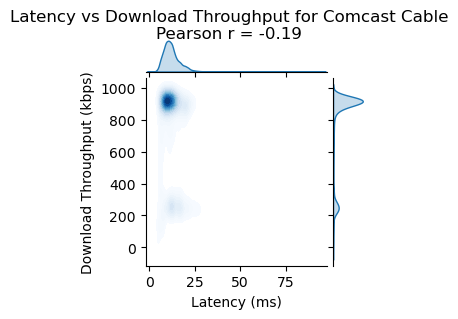
\includegraphics[width=\linewidth]{kde_down_boxplot_comcast.png}
        \caption{Comcast Cable}
    \end{subfigure}

    \begin{subfigure}{0.48\textwidth}
        \centering
        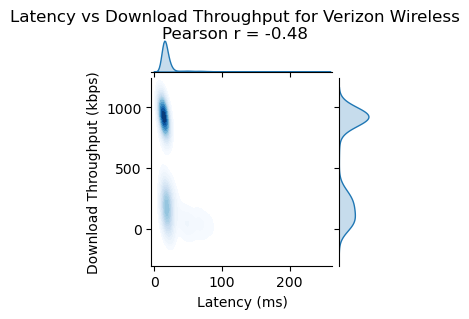
\includegraphics[width=\linewidth]{kde_down_boxplot_verizon.png}
        \caption{Verizon Wireless}
    \end{subfigure}
        
    \begin{subfigure}{0.48\textwidth}
        \centering
        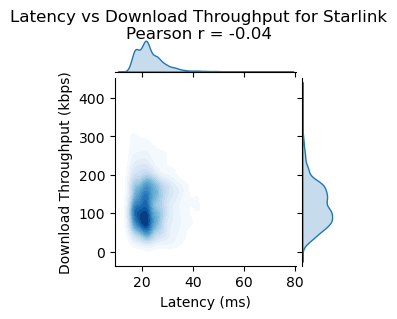
\includegraphics[width=\linewidth]{kde_down_boxplot_starlink.png}
        \caption{Starlink}
    \end{subfigure}

    \begin{subfigure}{0.48\textwidth}
        \centering
        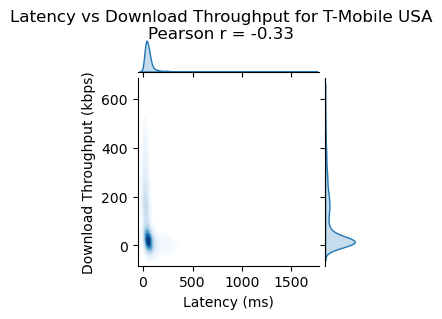
\includegraphics[width=\linewidth]{kde_down_boxplot_tmobile.png}
        \caption{T-Mobile USA}
    \end{subfigure}
    
    \caption{Kernel Density Estimate (KDE) distribution of download throughput versus latency. Outliers beyond the 97.5th percentile have been excluded to focus on the main distribution.}
    \label{fig:kde_download_throughput}
\end{figure}

Figure~\ref{fig:kde_download_throughput} shows latency vs. download throughput for the ISPs in this study. Comcast Cable, a wired network, exhibits a 
moderate negative correlation between latency and download throughput with a pearson r value of -0.19. High throughput is consistently achieved 
with relatively low latency (0–50 ms). Further, performance is concentrated around high throughput values, 
with a clear negative trend as latency increases. Starlink shows vey minimal correlation between 
latency and download throughput (Pearson r = -0.04). Throughput is highly variable and does not decrease 
significantly with increasing latency. This striking lack of correlation suggests that throughput alone 
does not capture network quality for Starlink. T-Mobile USA also demonstrates a weak negative correlation between latency 
and download throughput (Pearson r = -0.33). Latency is highly variable, reaching over 1000 ms in some cases, 
yet high throughput is still observed in a subset of measurements. The wide distribution of latency values demonstrates 
significant instabililty. Verizon Wireless has the strongest negative correlation between latency and download 
throughput (Pearson r = -0.48). Latency ranges from 0 to 200 ms, and although it demonstrates that higher latency 
reduces download throughput, high throughput is occasionally observed even at higher latencies.

\subsection{Upload Performance: Latency vs. Throughput}

\begin{figure}[H]
    \centering
    \begin{subfigure}{0.48\textwidth}
        \centering
        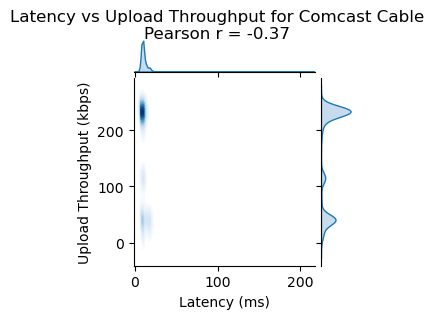
\includegraphics[width=\linewidth]{kde_up_boxplot_comcast.png}
        \caption{Comcast Cable}
    \end{subfigure}

    \begin{subfigure}{0.48\textwidth}
        \centering
        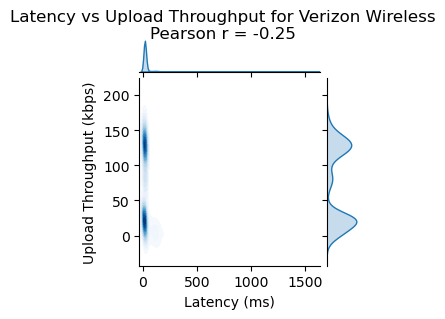
\includegraphics[width=\linewidth]{kde_up_boxplot_verizon.png}
        \caption{Verizon Wireless}
    \end{subfigure}
        
    \begin{subfigure}{0.48\textwidth}
        \centering
        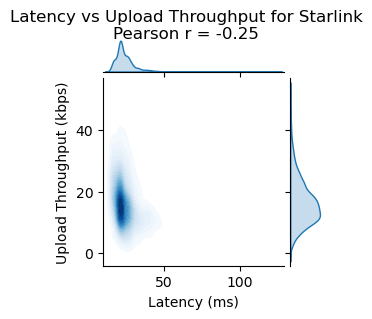
\includegraphics[width=\linewidth]{kde_up_boxplot_starlink.png}
        \caption{Starlink}
    \end{subfigure}

    \begin{subfigure}{0.48\textwidth}
        \centering
        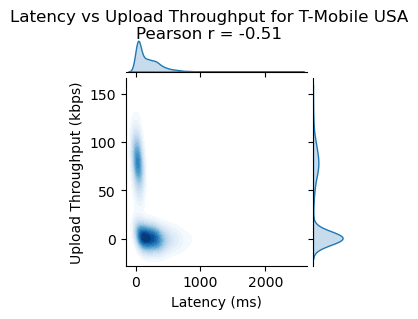
\includegraphics[width=\linewidth]{kde_up_boxplot_tmobile.png}
        \caption{T-Mobile USA}
    \end{subfigure}
    
    \caption{Kernel Density Estimate (KDE) distribution of upload throughput versus latency. Outliers beyond the 97.5th percentile have been excluded to focus on the main distribution.}
    \label{fig:kde_upload_throughput}
\end{figure}

Figure~\ref{fig:kde_upload_throughput} shows latency vs. upload throughput for the ISPs in this study.
Comcast Cable has a moderate negative correlation between latency and upload throughput (Pearson r = -0.37).
Similar to download throughput, high upload throughput is consistently achieved with low latency (0–50 ms).
The distribution is tightly concentrated, indicating stable performance. Starlink has a weak 
negative correlation between latency and upload throughput (Pearson r = -0.25).
Upload throughput is low and varies significantly with latency, reflecting instability again.
This variability is very pronounced. T-Mobile USA has a Pearson value of r = -0.51. 
Latency is highly variable, often exceeding 1000 ms, which severely impacts upload performance.
The wide distribution reflects quite poor and unstable performance, significantly impacted by 
poor latency. Verizon Wireless has a Pearson value of -0.25. The correlation is weak and 
the wide range of latency values (0–1500 ms) highlights the network's instability. 
High upload throughput is rarely achieved and there are many large latency spikes.


\subsection{Latency Characteristics}

\begin{figure}[H]
    \centering
    \begin{subfigure}{0.48\textwidth}
        \centering
        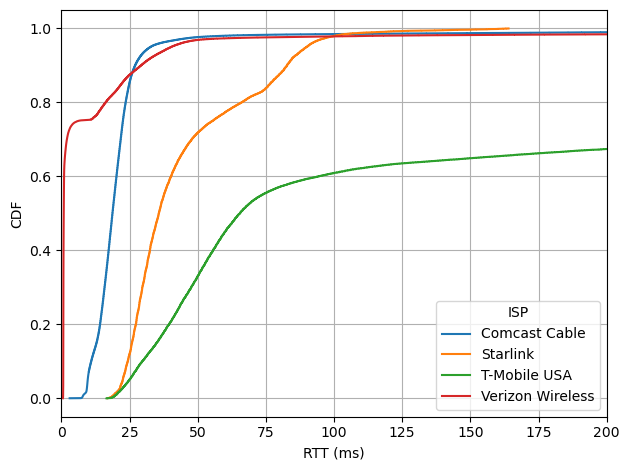
\includegraphics[width=\linewidth]{cdf_before_after.png}
        \caption{RTT Before and After Comparison}
        \label{fig:cdf_rtt_before_after}
    \end{subfigure}
    \hfill
    \begin{subfigure}{0.48\textwidth}
        \centering
        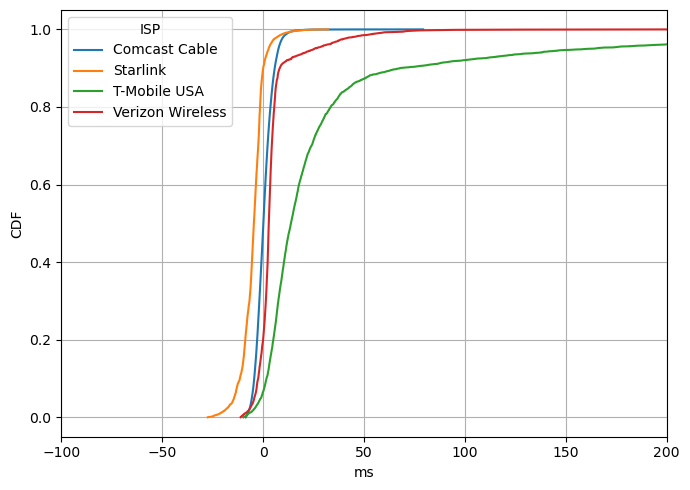
\includegraphics[width=\linewidth]{cdf_latency_down_difference.png}
        \caption{Download Latency - Ping Latency Difference}
        \label{fig:cdf_download_latency_difference}
    \end{subfigure}
    
    \begin{subfigure}{0.48\textwidth}
        \centering
        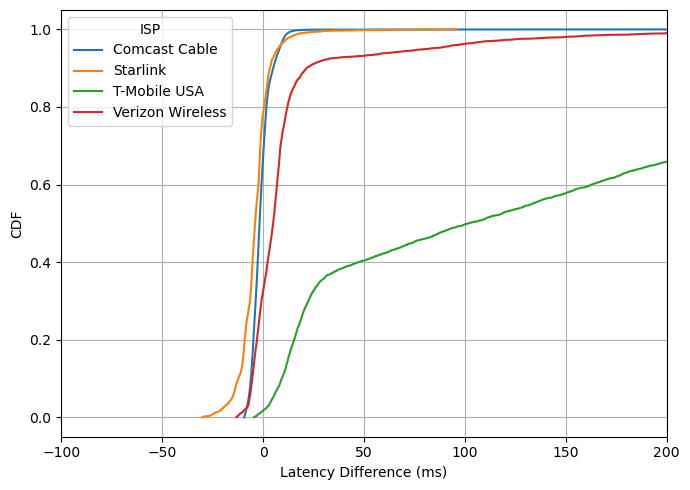
\includegraphics[width=\linewidth]{cdf_latency_up_difference.png}
        \caption{Upload Latency - Ping Latency Difference}
        \label{fig:cdf_upload_latency_difference}
    \end{subfigure}

    \caption{Cumulative Distribution Functions (CDFs) showing latency characteristics across ISPs. The top 1\% of latency differences (99th percentile) have been excluded for clarity.}
    \label{fig:cdf_latency_characteristics}
\end{figure}


Figure~\ref{fig:cdf_rtt_before_after} illustrates?? 

Figure~\ref{fig:cdf_download_latency_difference} visualizes the CDF of the difference 
between download latency and baseline ping latency for each ISP. Comcast shows minimal difference 
between download latency and ping latency, indicating stable performance. Fixed wireless networks 
display more differences. Starlink shows moderate variability, while T-Mobile and Verizon exhibit 
greater fluctuations. 

Figure~\ref{fig:cdf_upload_latency_difference} visualizes the CDF of the difference 
between upload latency and baseline ping latency for each ISP. Similar to download, 
Comcast maintains minimal variation between upload latency and ping latency. 
Verizon, and T-Mobile especially, show greater and steeper variance. 